\chapter{Preliminaries}
\label{chap:prelims}

\begin{quote} \small
	We discuss in brief the preliminaries that are used in our construction.
\end{quote}

\section{Metric spaces}
A metric space is a set $\msgspc$ along with a distance function $\mathsf{dis}: \msgspc \times \msgspc \rightarrow \RR^+$ such that distances are defined between all members of the set \cite{fuzzy}. In this paper, we will be using the \textit{Hamming metric}.
\subsection{Hamming Metric}
In this metric, $\msgspc = \bin^n$ and $\mathsf{dis}(w,w')$ is the number of positions in which strings $w$ and $w'$ differ.
\\ \\
We now define two functions $\mathsf{Diff}$ and $\mathsf{Comb}$.
\begin{itemize}
	\item[$\mathsf{Diff}$] - It takes as input two $n$-length messages $(w_1, w_2) \in \msgspc \times \msgspc$ and outputs the indices in which $w_1$ and $w_2$ differs. We will refer to this output as $\Delta$, i.e. $\mathsf{Diff}(w_1, w_2) = \Delta$. If the difference between $w_1$ and $w_2$ is bounded by $\tau$, then $|\Delta|$ can be bounded by $O{log(n) \cdot \tau}$.
	\item[$\mathsf{Comb}$] - It takes as inputs, $\Delta$ and a message $w_1 \in \msgspc$ and outputs $w_2 \in \msgspc$ such that $\mathsf{Diff}(w_1, w_2) = \Delta$
\end{itemize}

\section{Error-corecting codes}
We will not be using the traditional definition of codes in this.
We have an $(\msgspc, K, \tau)$ error correcting code. $\msgspc$ is the message space. The code $C$ is a subset of size $K$ of $\msgspc$. The error correcting distance of $C$, denoted by $\tau$, is the largest number $\tau > 0$ such that there is at most one valid code word $c \in C$ for a message $w$ such that $\mathsf{dis}(w,c) \leq \tau$. We denote the encoding and decoding funtions as $\mathsf{Enc}$ and $\mathsf{Dec}$ respectively.
\\ \\The encoding and decoding runs in polynomial time. Let $\mathsf{Dec}$ be the decoding function. We use the term decoding for the map that finds, given $w$, the $c \in C$ such that $\mathsf{dis}(w,c) \leq \tau$\cite{fuzzy} \footnote{For some messages $w$, a corresponding codeword $c$ may not exist, but when it exists it will be unique. We will, for the rest of this paper, assume that decoding always yields a codeword. The scheme can easily be adapted to handle cases when this doesn't happen, taking only a small hit in deduplication level. Decoding is not the inverse of encoding according to this definition. \cite{fuzzy}}.

\section{Randomness Extractors}
We have a family of extractors $\ext = \{\ext_{\secpar}\}$ where $\ext_{\lambda} : \bin^{s(\secpar)} \times \bin^{l(\secpar)} \rightarrow \bin^{\kappa(\secpar)}$. $s$ is the seed length, $l$ is the input length and $\kappa$ is the output length. $\ext_{\lambda}$ is an $(l,m,\kappa,\epsilon)$-strong extractor which means that for all min-entropy  $m$ distributions $W$ on $\bin^l$, $\textbf{SD}((\ext(W; X), X),$ $(U_\kappa,X )) \leq \epsilon $, where $X$ is uniform on $\bin^s$\cite{fuzzy}.

\subsection{MLE}    
The paper \cite{mle} introduced a new cryptographic primitive called MLE that 
enables secure deduplication.
An MLE scheme is a five-tuple of polynomial-time algorithms $\mathsf{MLE}=(\mathcal{P,K,E,D,T})$.
$\mathcal{D}$ and $\mathcal{T}$ are deterministic and the others are randomized.
\begin{displaymath}
\begin{aligned}
\text{Paramter Generation: \ \ \ } & P  \sample \mathcal{P}(1^{\lambda}) \\
\text{Key Generation: \ \ \ } & K  \sample \mathcal{K}_P(M) \\
\text{Encryption: \ \ \ } & C \sample \mathcal{E}_P (K,M) \\
\text{Decryption: \ \ \ } & \mathcal{D}_P (K,C) \in \{0,1\}^* \cup \{ \bot \} \\
\text{Tag Generation: \ \ \ } & T \leftarrow \mathcal{T}_P(C)
\end{aligned}
\end{displaymath}

There is a \textit{message space} associated with every lambda. 
\begin{equation}
\notag
MsgSp_{\mathsf{MLE}}(\lambda) \subseteq \{0,1\}^* \ \ \ \  \forall \lambda \in \mathbb{N}
\end{equation}	

\textit{Decryption Correctness: }
\begin{equation}
\notag
\mathcal{D}_P(K,C) = M\ \ \ \ \  \forall \lambda \in \mathbb{N} , \forall P \in [\mathcal{P}(1^\lambda)]
\end{equation}
\textit{Tag Correctness: } There exists a negligible function $\delta : \mathbb{N} \rightarrow [0,1]$ such that
$\forall \lambda \in \NN$, $P \in [P(\secparam)], \forall M \in$ MsgSp$_\mathsf{MLE}(\lambda)$
\begin{equation}
\notag
Pr[\mathcal{T}_P(C) \neq \mathcal{T}_P(C')] \leq \delta (\lambda)
\end{equation}
where $C \sample \mathcal{E}_P (\mathcal{K}_P(M),M) $ and $C' \sample \mathcal{E}_P (\mathcal{K}_P(M),M $ 
are ciphertexts of the same message.
\\
$\mathsf{MLE}$ is deterministic if $\mathcal{K}$ and $\mathcal{E}$ are deterministic. \\ \\
An MLE scheme exploits the fact that key is generated from the message and therefore people with identical messages will wnd up with identical ciphertexts. A tag is generated from ciphertext. Tags are used to compare different ciphertexts, and tags from different ciphertexts should only match if they are the same. Thus, tags enable comparison for the underlying messages. If a user uploads a ciphertext to a server and the tag of that ciphertext matches the tag of an existing file, then the server can identify that they are the same and thus need not store the redundant copy.

\subsubsection{Privacy for MLE}
Semantic security cannot be achieved using any MLE scheme. If the message space $\msgspc$ is predictable,
the adversary, given an encryption $C$ of $M$, can recover $M$ in $O(|\msgspc|)$ trials.\\
\begin{figure}[H]
	\centering
	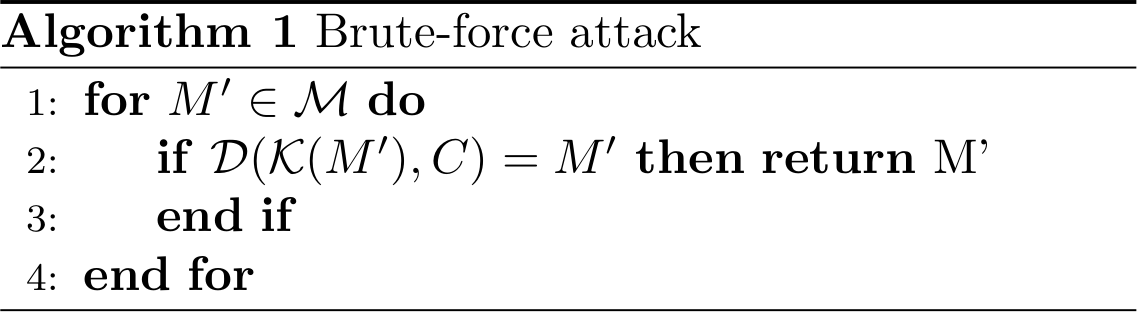
\includegraphics[scale=0.25]{brute}
\end{figure}
So MLE schemes are asked to have semantic security when the message space is unpredictable
\footnote{Unpredictability of message space is formalized later in section \ref{subsec:security}}. 
That is, messages have high min-entropy.

\subsection{Guessing Probability}
The guessing probability of a random variable $X$ is defined using the following equation
\begin{equation}
\textbf{GP}(X) = max_x \prob{X=x} = 2^{-H_\infty(X)}
\end{equation}


\subsection{Hash functions}
A hash function $\mathcal{H}: \bin^n \rightarrow \bin^m$ is a collision-resistant hash function if
\begin{itemize}
	\item $m < n$ and
	\item for all $\ppt \adv$, there exists a negligible function $\negl$ such that for all security parameters $\secpar \in \NN$,
	\begin{equation*}
	\mathsf{Pr} [ ( x_0, x_1) \leftarrow \adv ( \secparam, \mathcal{H} ): 
	x_0 \neq x_1 \wedge \mathcal{H} ( x_0 ) = \mathcal{H}(x_1) ] \leq \negl
	\end{equation*}
\end{itemize}
We denote the family of hash functions to be $\mathsf{H} = ( \mathcal{HK, H} )$

\section{Deterministic Symmetric Encryption}
Deterministic Symmetric Encryption scheme (D-SE), is defined as a pair of algorithms $\mathsf{SE=(E, D)}$. Encryption algorithm $\mathsf{E}$ takes as input the plaintext $m \in \bin^*$ and key $k \in \bin^{\kappa(\secpar)}$ and outputs the ciphertext $c \leftarrow \mathsf{E}(\secparam, k, m)$. Decryption returns the plaintext $m \leftarrow \mathsf{D}(\secparam, k, c)$. \cite{imle} We require D-SE scheme with CPA-security and key-recovery security (KR-secure). We say that a scheme is KR-secure if the probability that the adversary can guess the key from an encryption of a message of his choice is negligible.

\section{Immutability}
A table $T$ is said to be \textit{immutable} if no entry $T[t]$ can be changed once it is set. That is, once the table is initialized, values can only be assigned once \cite{imle}. An immutable table supports the set-iff-empty ($\mathsf{SiffE}$) operation which is defined as below. It takes as input, a table $T$, a message $m$ and an index $f$.

\begin{figure}[H]
	\centering
	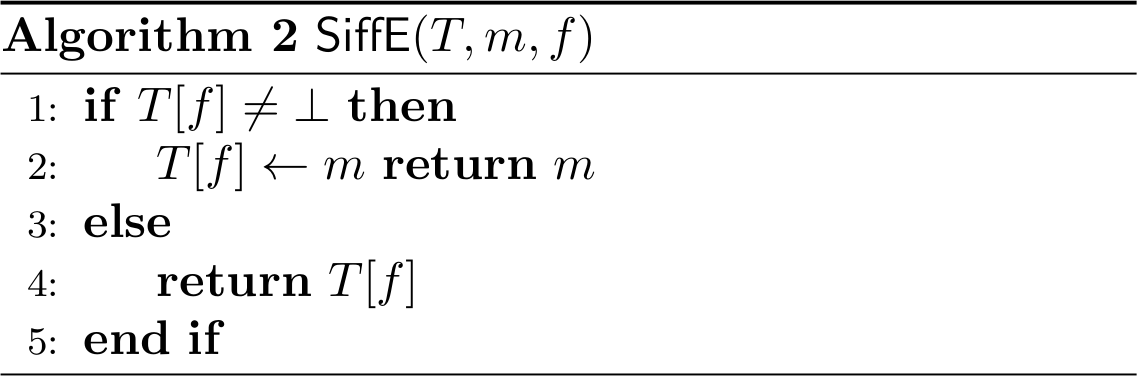
\includegraphics[scale=0.25]{SiffE}
\end{figure}


